

\begin{center}
\Huge
Optimering
\end{center}

\section*{Optimering}
\stepcounter{section}

Vi vil introducere dette emne med en række eksempler. 
\begin{exa}\label{exa:exa1}
Vi har $50m$ hegn og vi skal lave en indhegning til en gård. Vi vil gerne have, at arealet af indhegningen er maksimeret. En af indhegningens sider er op ad et hus, og vi vil gerne have en rektangulær indhegning. Derfor skal vi kun have tre sider i vores indhegning. Indhegningen kan ses på Figur \ref{fig:indh}
\begin{figure}[H]
\centering
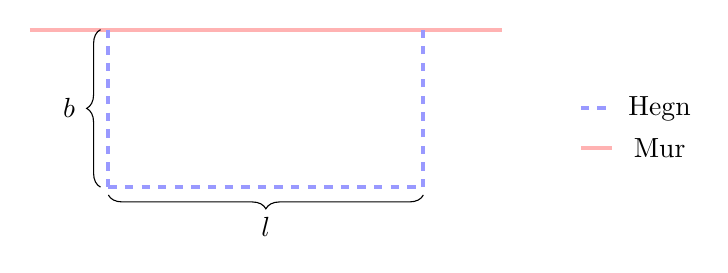
\begin{tikzpicture}
\draw[line width = 0.5mm,color=red!30] (-3,0) -- (3,0);
\draw[line width = 0.5mm, dashed, color = blue!40] (-2,0) -- (-2,-2);
\draw[line width = 0.5mm, dashed, color = blue!40] (-2,-2) -- (2,-2);
\draw[line width = 0.5mm, dashed, color = blue!40] (2,-2) -- (2,0);
\draw[line width = 0.5mm, dashed, color = blue!40] (4,-1) -- (4.4,-1);
\draw[line width = 0.5mm, color=red!30] (4,-1.5) -- (4.4,-1.5);
\node at (5,-1) {Hegn};
\node at (5,-1.5) {Mur};
\draw [decorate,decoration = {brace,mirror,amplitude = 5pt}] (-2.1,-0.0) --  (-2.1,-2);
\draw [decorate,decoration = {brace,mirror,amplitude = 5pt}] (-2,-2.1) --  (2,-2.1);
\node at (-2.5,-1) {$b$};
\node at (0,-2.5) {$l$};
\end{tikzpicture}
\caption{Hønsegård}
\label{fig:indh}
\end{figure}
Vi ved, at arealet af indhegningen er givet ved 
\begin{align}\label{eq:areal}
A(l,b) = lb,
\end{align}
samt at den samlede hegnslængde er givet ved 
\begin{align}\label{eq:hegnsl}
L(l,b) = 2b+l = 50m,
\end{align}
som er fastlagt til $50m$, da det er længden af det hegn, vi har til rådighed. Vi kan isolere længden $l$ i udtrykket \eqref{eq:hegnsl} som
\begin{align}\label{eq:lsomfb}
l = 50-2b.
\end{align}
Dette kan vi nu sætte ind i \eqref{eq:areal} for at få et udtryk for arealet $A(l,b)$, der kun afhænger af $b$:
\begin{align*}
A(l,b) = lb = (50-2b)b = 50b-2b^2.
\end{align*}
Grafen for $A(b)$ er tegnet i Figur \ref{fig:honsegraf}
\begin{figure}[H]
	\centering
	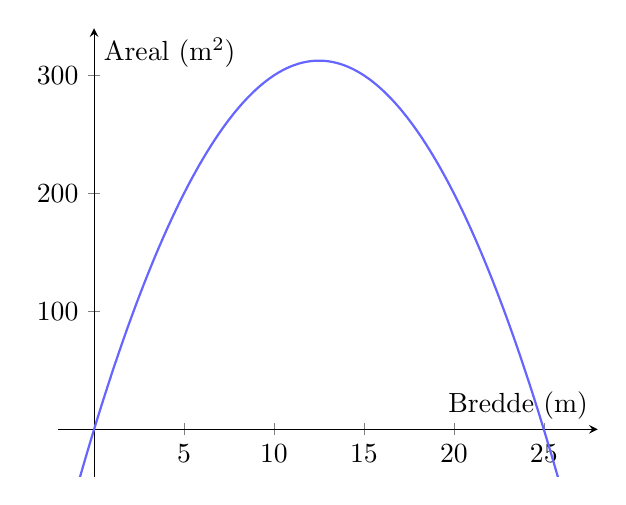
\begin{tikzpicture}
		\begin{axis}[
		axis lines = middle, 
		xmin = -2, xmax = 28, 
		ymin = -40, ymax = 340,
		xlabel = {Bredde (m)},
		ylabel = {Areal (m$^2$)}		
		]
			\addplot[color = blue!60, thick, samples = 1000, domain = -2:28] {50*x-2*x^2};
		\end{axis}
	\end{tikzpicture}
	\caption{Areal $A$ af hønsegård som funktion af bredde $b$.}
	\label{fig:honsegraf}
\end{figure}

Af Figur \ref{fig:honsegraf} ser det ud som om arealet er maksimeret omkring $b=12m$, men vi vil gerne finde den eksakte maksimerende bredde. Derfor vil vi finde toppunktet for andengradspolynomiet $A(b) = 50b-2b^2$. Vi finder derfor den afledede funktion
\begin{align*}
A'(b) = 50-4b,
\end{align*}
og vi sætter denne lig nul for at finde ud af, hvor tangenthældningen er $0$. Vi får altså
\begin{align*}
A'(b) = 50-4b = 0 &\Leftrightarrow 50=4b\\
&\Leftrightarrow 12,5=b,
\end{align*}
hvilket også stemmer nogenlunde overens med aflæsningen fra Figur \ref{fig:honsegraf}. Udtrykket \eqref{eq:lsomfb} giver os et udtryk for længden $l$ udtrykt ved bredden $b$. Altså må den maksimerende længde være 
\begin{align*}
l = 50-2\cdot 12,5 = 25m,
\end{align*}
altså skal længden af buret være $25m$ i det maksimerende tilfælde. Til slut bestemmer vi det maksimerende areal ved brug af \eqref{eq:areal} som
\begin{align*}
A((12,5),25) = 12,5\cdot25 = 312,5m^2,
\end{align*}
som altså er det maksimalt opnåelige areal til hønseindhegningen. 
\end{exa}
\begin{exa}
Vi forestiller os, at vi har en kasse med kvadratisk bund med areal $b^2$ og højde $h$. Vi ønsker at minimere materialeforbruget til kassen, når kassen ikke skal have et låg, og rumfanget af kassen skal være $4m^3$. Kassen kan ses på Figur \ref{fig:kasse}
\begin{figure}[H]
\centering
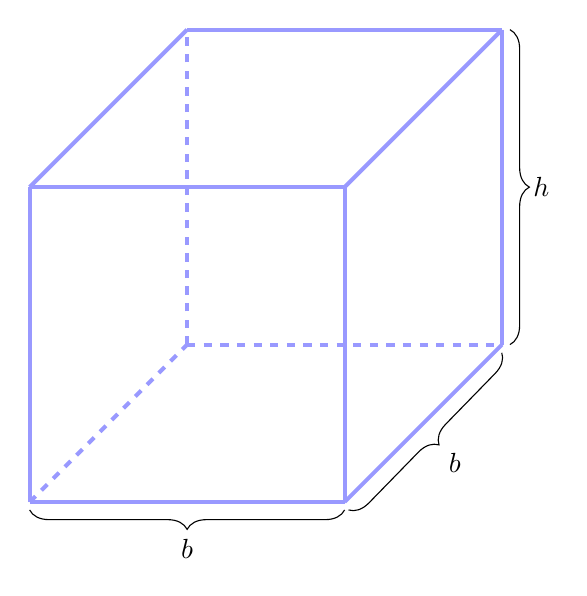
\begin{tikzpicture}
\draw[line width = 0.5mm,  color = blue!40] (0,0) -- (0,4);
\draw[line width = 0.5mm,  color = blue!40] (0,0) -- (4,0);
\draw[line width = 0.5mm,  color = blue!40] (4,0) -- (4,4);
\draw[line width = 0.5mm,  color = blue!40] (0,4) -- (4,4);

\draw[line width = 0.5mm,  color = blue!40] (0,4) -- (2,6);
\draw[line width = 0.5mm,  color = blue!40] (4,4) -- (6,6);
\draw[line width = 0.5mm,  color = blue!40] (6,6) -- (6,2);

\draw[line width = 0.5mm,  color = blue!40] (4,0) -- (6,2);
\draw[line width = 0.5mm,  color = blue!40] (2,6) -- (6,6);

\draw[line width = 0.5mm, dashed,  color = blue!40] (0,0) -- (2,2);
\draw[line width = 0.5mm, dashed,  color = blue!40] (2,2) -- (2,6);
\draw[line width = 0.5mm, dashed,  color = blue!40] (2,2) -- (6,2);

\draw [decorate,decoration = {brace,mirror,amplitude = 7pt}] (0,-0.1) --  (4,-0.1);
\draw [decorate,decoration = {brace,mirror,amplitude = 7pt}] (4.05,-0.1) --  (6,1.9);
\draw [decorate,decoration = {brace,mirror,amplitude = 7pt}] (6.1,2) --  (6.1,6);

\node at (2,-0.6) {$b$};
\node at (5.4,0.5) {$b$};
\node at (6.5,4) {$h$};
\end{tikzpicture}
\caption{Kasse uden låg med højde $h$ og grundfladeareal $b^2$.}
\label{fig:kasse}
\end{figure}
Fremgangsmåden er tilsvarende den, vi opstillede til eksemplet med hønsegården. Vi opstiller altså de variabelsammenhænge, vi har. Det samlede overfladeareal er givet ved
\begin{align*}
O(b,h) = b^2+4bh,
\end{align*}
hvilket er størrelsen, vi skal minimere. Kassens rumfang er givet ved
\begin{align*}
R(b,h) = b^2h = 4.
\end{align*}
Vi kan isolere $h$ i dette udtryk og få
\begin{align*}
h = \frac{4}{b^2}.
\end{align*}
Dette sættes ind i udtrykket for det samlede overfladeareal:
\begin{align*}
O(b,h) = b^2+ 4bh = b^2 + \frac{4\cdot4b}{b^2} = b^2+\frac{16}{b}.
\end{align*}
Dette skal vi maksimere. Grafen for $O(b)$ kan ses på Figur \ref{fig:kassegraf}.
\begin{figure}[H]
	\centering
	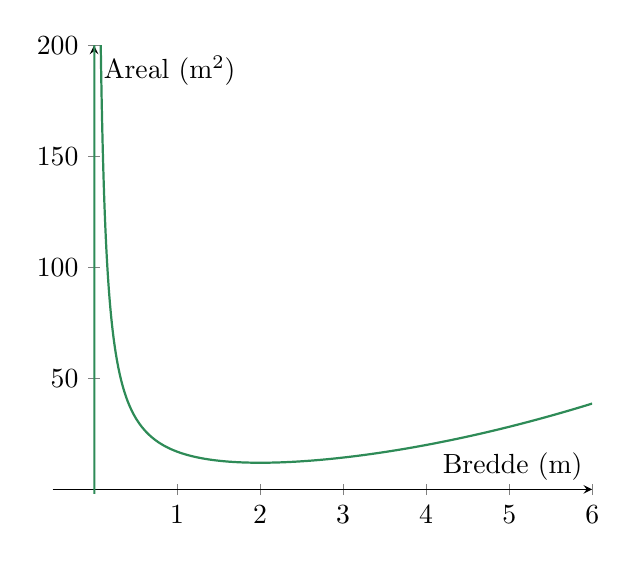
\begin{tikzpicture}
		\begin{axis}[
		axis lines = middle, 
		xmin = -0.5, xmax = 6, 
		ymin = -2, ymax = 200,
		xlabel = {Bredde (m)},
		ylabel = {Areal (m$^2$)}		
		]
			\addplot[color = SeaGreen, thick, samples = 1000, domain = -0.2:6] {x^2+16/x};
		\end{axis}
	\end{tikzpicture}
	\caption{Overfladeareal $O$ som funktion af bredde $b$.}
	\label{fig:kassegraf}
\end{figure}

Af grafen kan det ses, at der er et lokalt minimum omkring en bredde $b=2m$. Vi ønsker som før at finde punktet, hvor tangenthældningen er $0$, så vi differentierer overfladearealet og sætter lig $0$:
\begin{align*}
O'(b) = 2b-\frac{16}{b^2}=0&\Leftrightarrow 2b^3-16=0\\
						&\Leftrightarrow 2b^3 = 16\\
						&\Leftrightarrow b^3 = 8\\
						&\Leftrightarrow b = \sqrt[3]{8} = 2,
\end{align*}
og den bredde $b$, der minimerer overfladearealet er $b=2m$. Da $h=4/b^2$, så er den minimerende højde $h=4/2^2=1m$ og det minimerede overfladeareal er givet ved
\begin{align*}
O(2,1) = 2^2+4\cdot 2\cdot 1 = 12m^2
\end{align*}
\end{exa}

\subsection*{Opgave 1}

Løs problemet med hønseburet fra Eksempel \ref{exa:exa1}, men nu hvor den samlede længde på hegnet er $20m.$

\subsection*{Opgave 2}
En landmand skal have lavet en indhegning til en mark. Han har 5000m hegn og indhegningen skal være rektangulær. Hvor bred og lang skal indhegningen være, for at indhegningens areal er maksimeret?

\subsection*{Opgave 3}
Vi skal producere en cylindrisk dåse til en producent af dåsetomater. Vi skal have et rumfang på 0.5L og dåsens materialeforbrug skal være minimeret. Optimér derfor dåsens højde og radius så overfladearealet bliver minimalt. 

\subsection*{Opgave 4}
Vi skal konstruere en beholder til en pindeis. Den skal være cylindrisk og den skal have et låg som en halvkugle. Vi kan se en illustration af beholderen på Figur \ref{fig:pindeis}.
\begin{figure}[H]
	\centering
	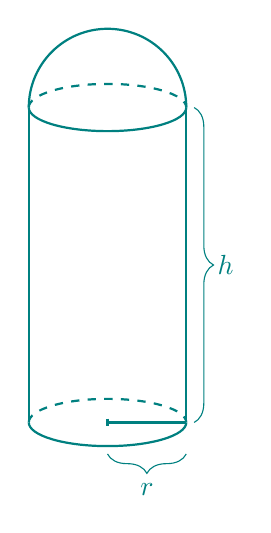
\begin{tikzpicture}  
		%Sides
		\draw[color = teal, thick] (0,0) -- (0,4);
		\draw[color = teal, thick] (2,0) -- (2,4);
		%Buttom and top
		\draw[color = teal, thick] (0,0) arc [start angle = 180, end angle = 360,
		 x radius = 1cm, y radius = 0.3cm];
		\draw[color = teal, thick, dashed] (0,0) arc [start angle = 180, end angle = 0,
		 x radius = 1cm, y radius = 0.3cm]; 
		 \draw[color = teal, thick] (0,4) arc [start angle = 180, end angle = 360,
		 x radius = 1cm, y radius = 0.3cm];
		\draw[color = teal, thick, dashed] (0,4) arc [start angle = 180, end angle = 0,
		 x radius = 1cm, y radius = 0.3cm]; 
		 %Half-ball
		 \draw[color = teal, thick] (0,4) arc [start angle = 180, end angle = 0, radius = 1cm];
		 %Braces
		 \draw[decorate,decoration = {brace,amplitude = 7pt, mirror},color = teal] (2.1,0) -- (2.1,4);
		 \node[color = teal] at (2.5,2) {$h$};
		 \draw[decorate,decoration = {brace,amplitude = 7pt, mirror},color = teal] (1,-0.4) -- (2,-0.4);
		 \node[color = teal] at (1.5,-0.85) {$r$};
		 \draw[color = teal, thick] (2,0) -- (1,0);
		 \draw[color = teal, thick] (1,0.05) -- (1,-0.05);
	\end{tikzpicture}
	\caption{Beholder til is.}
	\label{fig:pindeis}
\end{figure}

Beholderen skal have en bund, en side og låget, der alle er i samme materiale. Den skal indeholde 150 mL is, og rumfanget skal være så småt som muligt. 

\begin{enumerate}[label=\roman*)]
	\item Bestem et udtryk for rumfanget og sæt dette lig 150.
	\item Bestem et udtryk for overfladearealet og brug i) til at minimere det. 
\end{enumerate}


\subsection*{Opgave 5}
Vi skal tegne et hus i profil i en dystopisk fremtid, hvor blyanter er rationerede. Det skal have et areal på 40 kvadratcentimeter og det skal bestå af et rektangel i bunden og en ligebenet trekant i toppen. Taget skal have en vinkel på 45 grader. Da blyanter ikke er frit tilgængelige, skal vi bruge så lidt streg som muligt. Optimér derfor omkredsen af huset. 


\newpage

\subsection*{Opgave 6}
Vi skal bygge en pyramide, og vi har sten nok til at overfladearealet af pyramiden kan blive 1 km$^2$. Vi vil gerne have at pyramiden har kvadratisk bund, og vi ønsker, at rumfanget af pyramiden er så stort som muligt, og vi ønsker ikke, at der skal være bund i pyramiden. Bredden og længden af pyramiden er $x$ og højden af pyramiden er $h$. Pyramiden kan ses på Figur \ref{fig:pyramide2}
\begin{figure}[H]
\centering
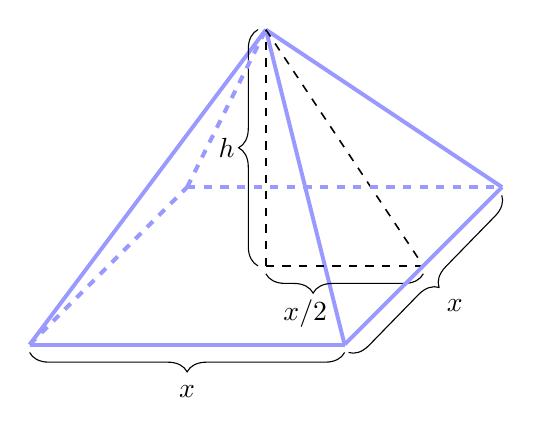
\begin{tikzpicture}
\draw[line width = 0.5mm,  color = blue!40] (0,0) -- (4,0);
\draw[line width = 0.5mm,  color = blue!40] (0,0) -- (3,4);
\draw[line width = 0.5mm,  color = blue!40] (4,0) -- (3,4);
\draw[line width = 0.5mm,  color = blue!40] (6,2) -- (3,4);

\draw[line width = 0.2mm, dashed] (3,1) -- (3,4);
\draw[line width = 0.2mm, dashed] (3,1) -- (5,1);
\draw[line width = 0.2mm, dashed] (3,4) -- (5,1);

\draw[decorate,decoration = {brace,amplitude = 7pt}] (3-0.1,1) -- (3-0.1,4);
\draw[decorate,decoration = {brace,mirror,amplitude = 7pt,aspect = 0.3}] (3,1-0.1) -- (5,1-0.1);

\draw[line width = 0.5mm,  color = blue!40] (4,0) -- (6,2);

\draw[line width = 0.5mm, dashed,  color = blue!40] (0,0) -- (2,2);
\draw[line width = 0.5mm, dashed,  color = blue!40] (2,2) -- (6,2);
\draw[line width = 0.5mm, dashed,  color = blue!40] (2,2) -- (3,4);



\draw [decorate,decoration = {brace,mirror,amplitude = 7pt}] (0,-0.1) --  (4,-0.1);
\draw [decorate,decoration = {brace,mirror,amplitude = 7pt}] (4.05,-0.1) --  (6,1.9);


\node at (2,-0.6) {$x$};
\node at (5.4,0.5) {$x$};
\node at (2.5,2.5) {$h$};
\node at (3.5,0.4) {$x/2$};
\end{tikzpicture}
\caption{Pyramide med kvadratisk bund}
\label{fig:pyramide2}
\end{figure}
\begin{enumerate}[label=\roman*)]
\item Rumfanget af en pyramide er givet ved $R = (b\cdot l\cdot h)/3$, hvor $l$ er længden af pyramiden, $b$ er bredden af pyramiden og $h$ er højden af pyramiden. Bestem rumfanget af pyramiden på Figur \ref{fig:pyramide2}.
\item Argumentér for, at overfladeareal af en af de fire sidetrekanter er givet ved 
\begin{align*}
O_T = \frac{x\sqrt{\frac{x^2}{4}+h^2}}{2},
\end{align*}
og konkludér, at det samlede overfladeareal af pyramiden må være givet ved 
\begin{align*}
O_P = 2 x \sqrt{\frac{x^2}{4}+h^2}.
\end{align*}

\item Udnyt, at vi ved, at det samlede overfladeareal skal være $1$km$^2$, således at 
\begin{align*}
O_P = 1 = 2 x \sqrt{\frac{x^2}{4}+h^2},
\end{align*}
og brug dette til at vise, at 
\begin{align*}
h=\sqrt{\frac{1}{4 x^2}-\frac{x^2}{4}}.
\end{align*}

\item Indsæt nu udtrykket for $h$ i udtrykket for rumfanget af pyramiden og plot rumfanget som funktion af $x$ på intervallet $[0,1]$. 
\item Bestem de dimensioner på pyramiden, der gør rumfanget af pyramiden maksimalt.
\end{enumerate}